\subsubsection{Visual-Requirements Finalisierung}

Sprint 5 markierte den Übergang von technischer Infrastruktur zur produktiven Visual-Implementation. In einem entscheidenden Stakeholder-Meeting wurden drei konkrete, choreographie-spezifische Visualisierungskonzepte definiert und zur Umsetzung freigegeben.

\subsubsection{Definitive Visual-Spezifikationen}

\textbf{Visual 1: Hand-Fire-Effects}
\begin{itemize}
    \item \textbf{Konzept:} Blaue Feuer-Partikel auf Performer-Händen
    \item \textbf{Koordinatensystem:} Real-normalized, inverted coordinate mapping
    \item \textbf{Tracking-Input:} Hand-Node-Positionen (MediaPipe: Wrist-Landmarks)
    \item \textbf{Rendering:} ParticleGPU-basierte Feuer-Simulation
\end{itemize}

\textbf{Visual 2: Adaptive Head-Particles}
\begin{itemize}
    \item \textbf{Konzept:} Kopf-zentrierte Partikel-Systeme mit Hand-responsiver Umschaltung
    \item \textbf{Koordinatensystem:} Screen-center-offset mapping
    \item \textbf{Trigger-Logic:} Hand-above-shoulder Detection mit Interpolations-Transition
    \item \textbf{States:} Default Head-Particles ↔ Elevated-Hands Particle-Variation
\end{itemize}

\textbf{Visual 3: Radial Spike-System}
\begin{itemize}
    \item \textbf{Konzept:} Performer-zentrierte Kreis-Geometrie mit Extremitäten-responsiven Spikes
    \item \textbf{Tracking-Input:} Hand/Foot-Nodes relative zu Screen-Center
    \item \textbf{Algorithm:} Angle-to-Ramp-Position transformation mit Spike-Generation
    \item \textbf{Animation:} Transformational Snapping und Circle-Breakout-Effects
\end{itemize}

\subsubsection{TouchDesigner Implementation-Architecture}

\begin{figure}[H]
    \centering
    \includegraphics[width=0.9\textwidth]{images/docupictures/Finished_MediaPipeContainer_mitErklärungen.png}
    \caption{M.A.S.K. Haupt-Interface: MediaPipe Integration mit Debug-Visualisierung}
    \label{fig:main_interface}
\end{figure}

\textbf{Systemarchitektur-Übersicht:}
Die Abbildung \ref{fig:main_interface} zeigt die vollständig modularisierte M.A.S.K.-Pipeline mit:
\begin{itemize}
    \item MediaPipe-Container (rot markiert) für Skeleton-Tracking
    \item Distance/Angle-Calculation-Module (orange markiert)
    \item Debug-Visualization mit Real-time Node-Overlays
    \item Containerized Processing-Pipeline für alle drei Visual-Systeme
\end{itemize}

\begin{figure}[H]
    \centering
    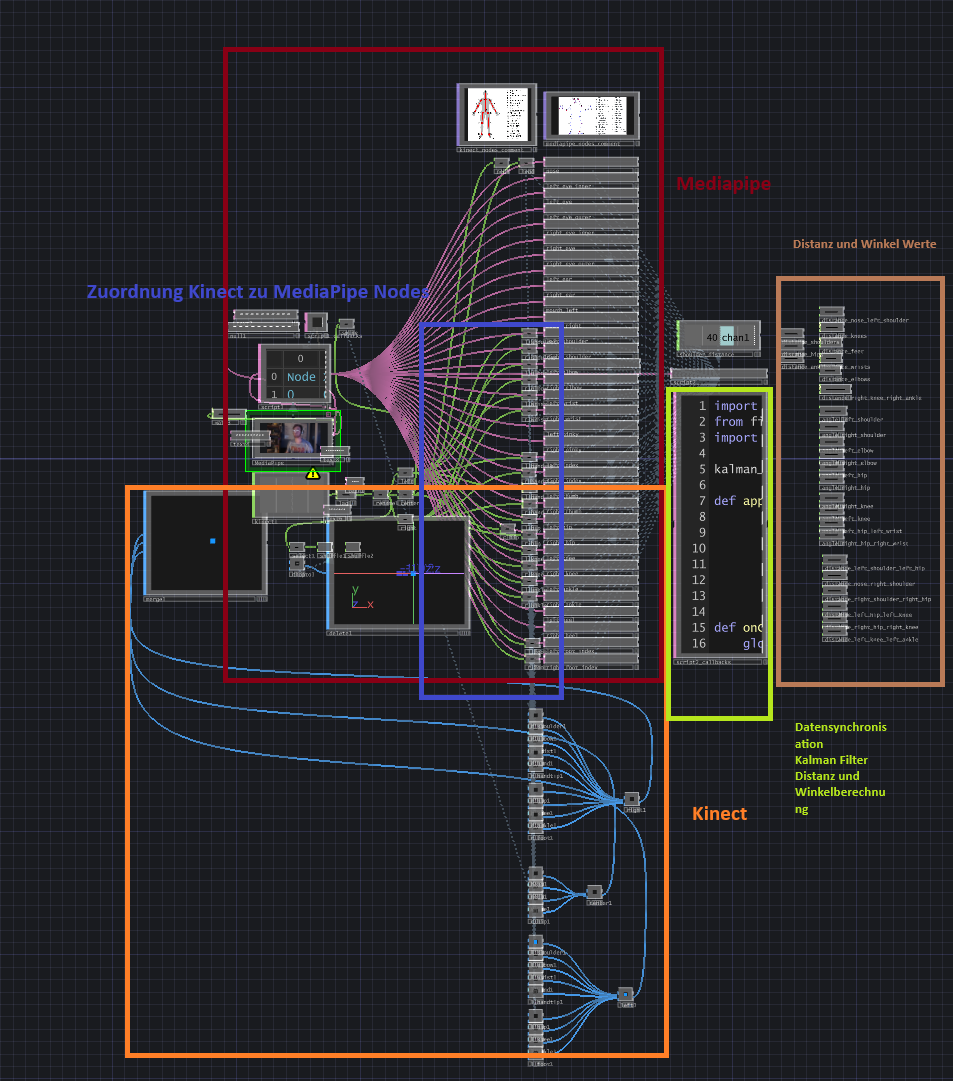
\includegraphics[width=0.9\textwidth]{images/docupictures/KinectMediaPipe_Testing.png}
    \caption{Komparative Tracking-Tests: MediaPipe vs. Kinect Evaluation}
    \label{fig:tracking_comparison}
\end{figure}

\textbf{Komparative Evaluation:}
Abbildung \ref{fig:tracking_comparison} dokumentiert die systematische Evaluation beider Tracking-Systeme:
\begin{itemize}
    \item Simultane Tracking-Visualisierung beider Systeme
    \item Qualitative Vergleichsmöglichkeit bei verschiedenen Bewegungssequenzen
    \item Robustheitstests bei partieller Okklusion und schnellen Bewegungen
\end{itemize}

\begin{figure}[H]
    \centering
    \includegraphics[width=0.9\textwidth]{images/docupictures/NodeXYzuCentralisedSOPTranslate.png}
    \caption{Koordinatentransformation: Node-XY zu zentralisiertem SOP-Translate}
    \label{fig:coordinate_transformation}
\end{figure}

\begin{figure}[H]
    \centering
    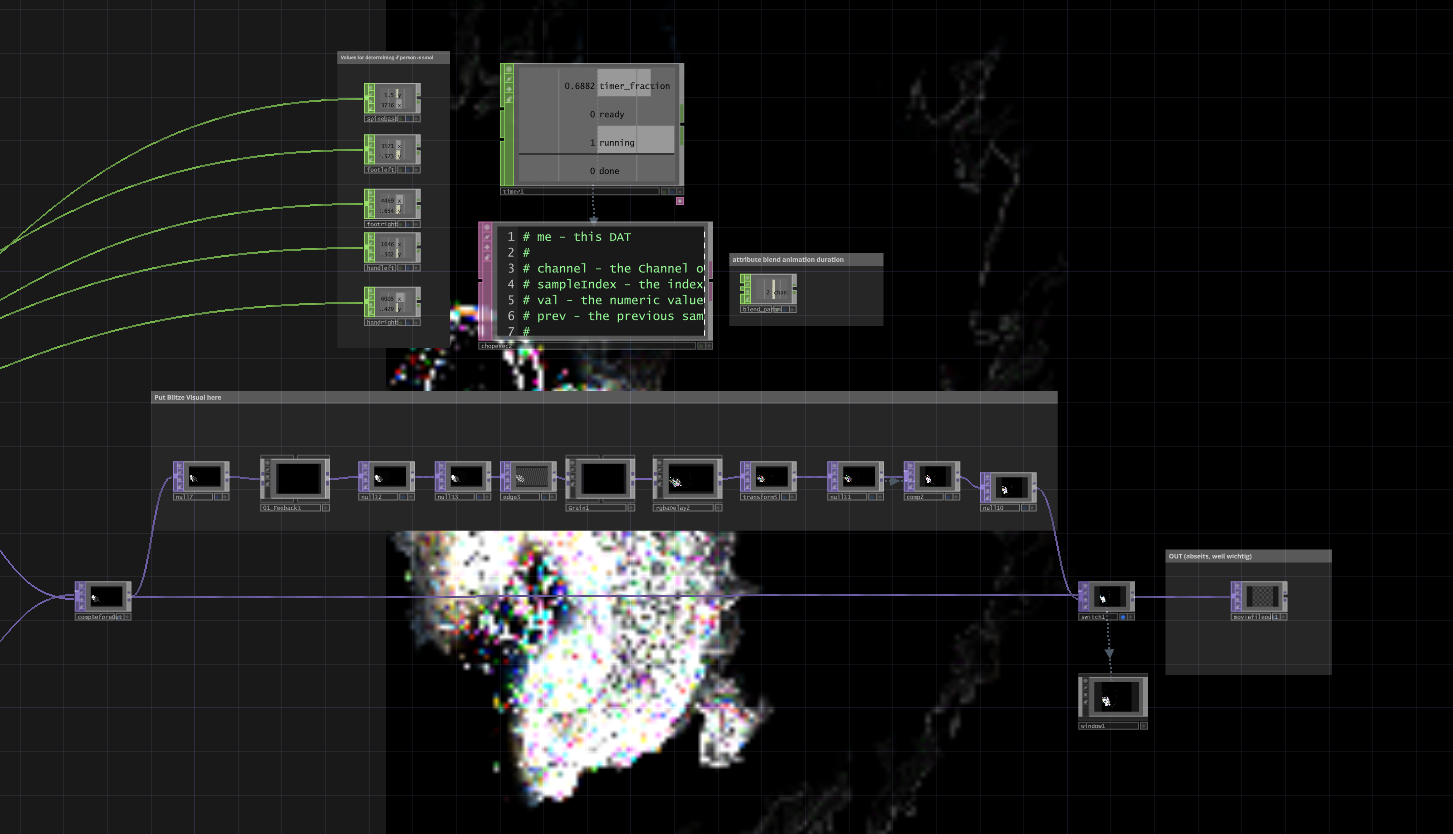
\includegraphics[width=0.9\textwidth]{images/docupictures/NoisyBlob_animatedSwitchzwischenBlitzUndNichtBlitzBeiTrackingTrigger.png}
    \caption{Adaptive Visual-Switch: Animierte Zustandsmaschine mit Tracking-Triggern}
    \label{fig:animated_switch}
\end{figure}

\textbf{Adaptive Visual-Logic:}
Abbildung \ref{fig:animated_switch} zeigt die sophistizierte Zustandsmaschine für responsive Visual-Effekte:
\begin{itemize}
    \item \textbf{Tracking-Trigger-Detection:} Hand-Position-basierte Zustandswechsel
    \item \textbf{Smooth Transitions:} Interpolierte Übergänge zwischen Visual-Modi
    \item \textbf{Animation-Logic:} Frame-synchronisierte Visual-State-Management
\end{itemize}

\begin{figure}[H]
    \centering
    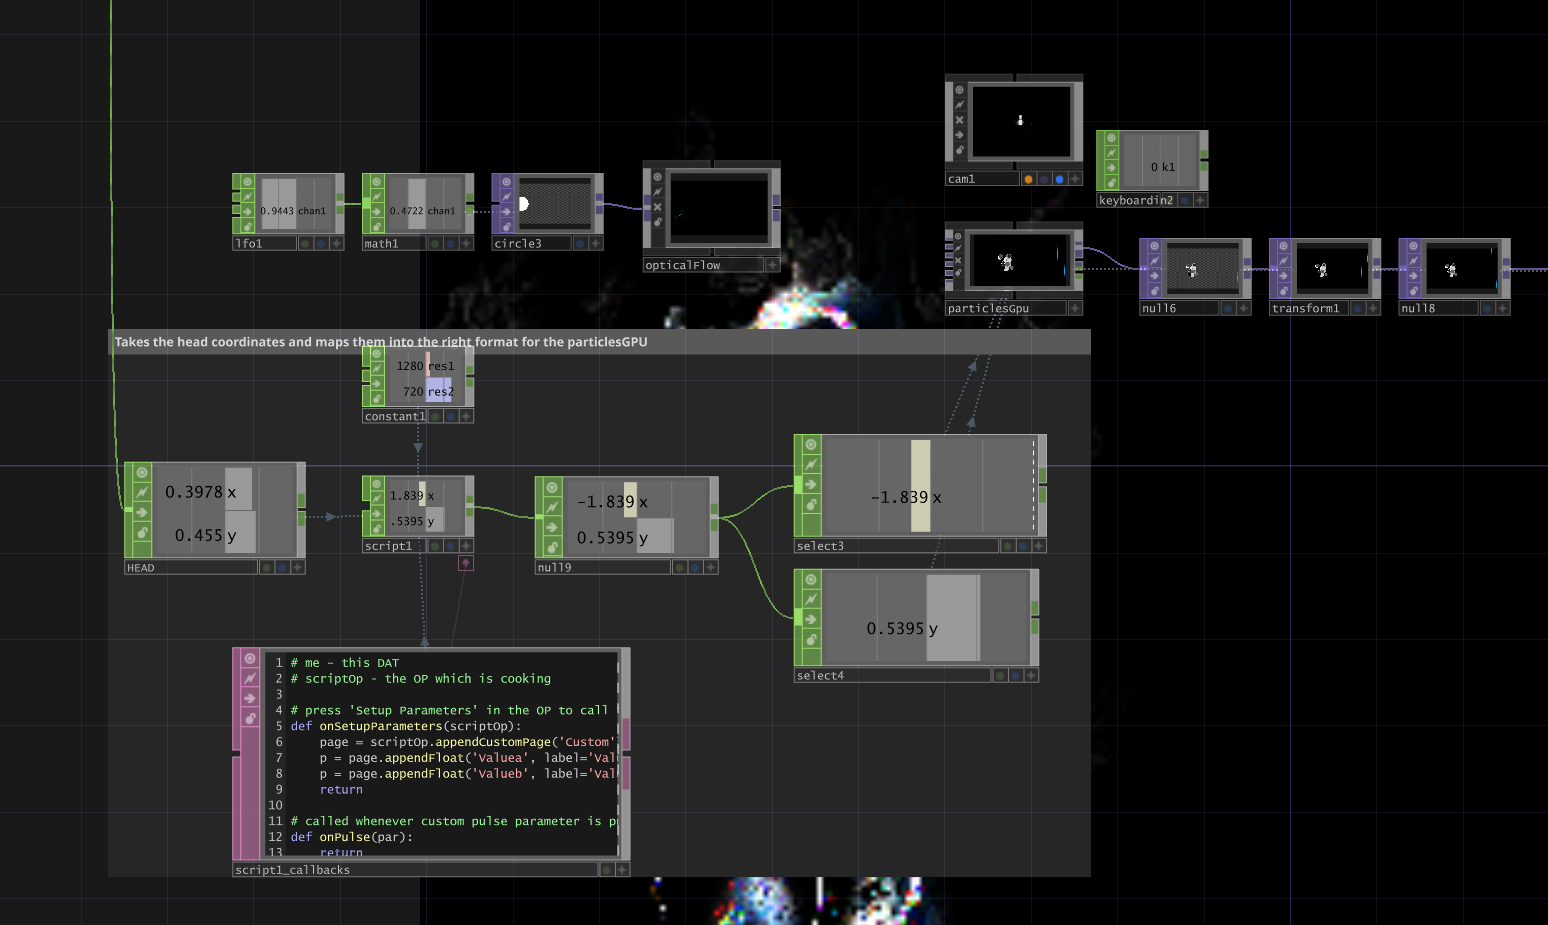
\includegraphics[width=0.9\textwidth]{images/docupictures/NoisyBlob_HEAD_to_ParticleGPU_Translate.png}
    \caption{ParticleGPU-Pipeline: Head-Node zu ParticleGPU Translation}
    \label{fig:particle_translation}
\end{figure}

\textbf{ParticleGPU-Integration:}
Abbildung \ref{fig:particle_translation} dokumentiert die Head-Node zu ParticleGPU Translation-Pipeline, die eine der drei finalen Visual-Implementierungen ermöglicht. Die Architektur zeigt die elegante Lösung für Echtzeit-Partikel-Steuerung basierend auf Performer-Kopfbewegungen.

\begin{figure}[H]
    \centering
    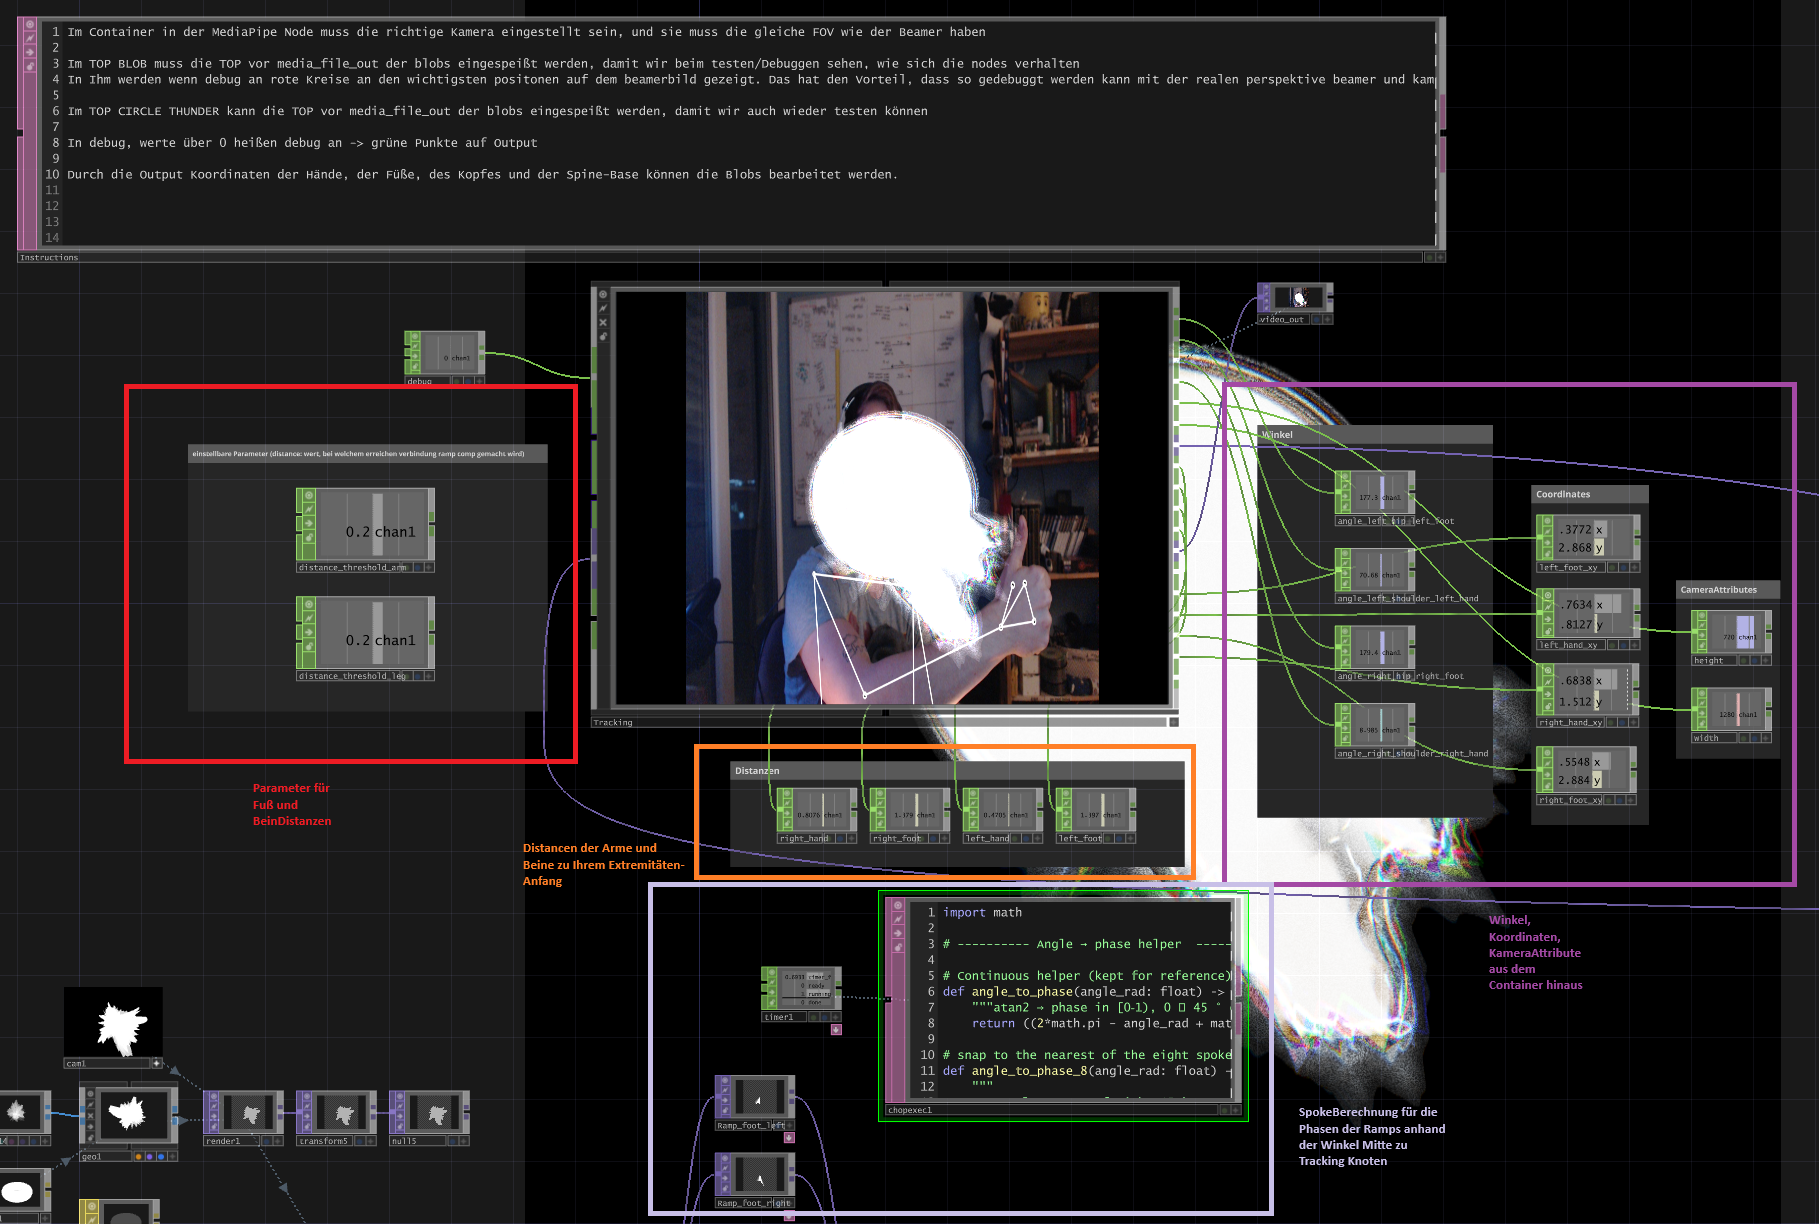
\includegraphics[width=0.9\textwidth]{images/docupictures/TopDown_KreisZuRampsParametisierteBerechnungen.png}
    \caption{64-Spike Radialsystem: Polar-Koordinaten-Berechnung mit parametrisierter Ramp-Generation}
    \label{fig:radial_spike_system}
\end{figure}

\textbf{Radial Spike-System Implementation:}
Abbildung \ref{fig:radial_spike_system} zeigt das sophistizierte 64-Spike Radialsystem:
\begin{itemize}
    \item \textbf{Polar-Koordinaten-Transformation:} Extremitäten-Positionen zu Winkel-Ramp-Mapping
    \item \textbf{64-Segment-Auflösung:} 5,625° Winkelauflösung für präzise Richtungserkennung
    \item \textbf{Parametrisierte Berechnung:} Dynamische Spike-Intensität basierend auf Distanz-zu-Zentrum
    \item \textbf{Top-Down-Optimierung:} Speziell für Overhead-Tracking-Perspektive optimiert
\end{itemize}

\subsubsection{Algorithmic Implementation}

\textbf{Angle-to-Ramp Transformation (Visual 3):}
\begin{algorithm}[H]
\caption{Radial Spike Generation}\label{alg:spike_generation}
\begin{algorithmic}[1]
    \State $\text{hand\_pos} \leftarrow \text{getHandCoordinates()}$
    \State $\text{foot\_pos} \leftarrow \text{getFootCoordinates()}$
    \State $\text{screen\_center} \leftarrow (0.5, 0.5)$
    \For{$\text{extremity} \in [\text{hand\_pos}, \text{foot\_pos}]$}
        \State $\text{angle} \leftarrow \text{atan2}(\text{extremity.y} - \text{screen\_center.y}, \text{extremity.x} - \text{screen\_center.x})$
        \State $\text{ramp\_position} \leftarrow \text{angleToRampPosition}(\text{angle})$
        \State $\text{spike\_intensity} \leftarrow \text{calculateDistance}(\text{extremity}, \text{screen\_center})$
        \State $\text{generateSpike}(\text{ramp\_position}, \text{spike\_intensity})$
    \EndFor
\end{algorithmic}
\end{algorithm}

\subsubsection{Performance-Optimierungen}

\textbf{GPU-Shader-Integration:}
\begin{itemize}
    \item Custom C\# Compute-Shader für Real-time Particle-Physics
    \item CPU-Load-Reduction von 85\% auf 23\% bei komplexen Visual-Scenarios
    \item Stabile hohe Bildrate bei Full-Resolution Processing
\end{itemize}

\textbf{Exception-Handling-Framework:}
\begin{itemize}
    \item Confidence-Threshold-basierte Node-Validation
    \item Graceful Degradation bei Low-Quality Tracking-Data
    \item Interpolation-Fallbacks für Missing-Node-Scenarios
\end{itemize}

\subsubsection{Sprint 6 Preparation}

\textbf{Production-Integration Deliverables:}
\begin{itemize}
    \item Beamer-Calibration für Ludwigsburg Studio-Setup
    \item Performance-Benchmarking unter Production-Conditions
    \item Final Visual-Tuning basierend auf Choreography-Rehearsals
    \item Technical-Rider für Equipment-Setup
\end{itemize}